\documentclass[12pt]{article}
\usepackage[a4paper, total={7in, 10in}]{geometry}
\usepackage{amsmath}
\usepackage{graphicx}

\title{Week 6 Problem Set: CSIMC Preparation\vspace{-3mm}}
\author{2018-2019 SLSS Math Club\vspace{-5mm}}
\date{November 14, 2018\vspace{-5mm}}

\newcommand{\bspace}{\\ \\ \\ \\ \\ \\ \\ \\}
\newcommand{\interspace}{\\ \\ \\ \\ \\ \\ \\ \\}

\begin{document}
\maketitle

\section*{Basic Problems}
\begin{enumerate}
    \item In the diagram, point $D$ is on $AC$ so that $BC$ is perpendicular to $AC$. Also, $AB = 13, BC = 12\sqrt{2},$ and $BD=12$. What is the length of $AC$? \\ 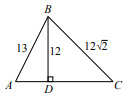
\includegraphics[scale = 1.85]{Graphics/Week_6/d2.PNG}
    
    \item In the diagram, $ABCD$ is a square with side length $8$cm. Point $E$ is on $AB$ and point $F$ is on $DC$ so that $\Delta AEF$ is right angled at $E$. If the area of $AEF$ is $30\%$ of the area of $ABCD$, what is the length of $AE$? \\ 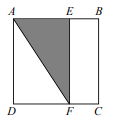
\includegraphics[scale = 1.85]{Graphics/Week_6/d1.PNG}
    
    \item What is the value of $\Large(\sqrt{4 + \sqrt{4}} \Large)^4$? \bspace
    
    \item There is exactly one pair of $(x, y)$ positive integers for which $\sqrt{23 - x} = 8 - y^2$. What is this pair $(x, y)$?
\end{enumerate} \newpage

\section*{Intermediate Problems}
\begin{enumerate}
    \item Determine all real numbers $x$ for which $x^4 - 3x^3 + x^2 - 3x = 0$. \interspace
    
    \item The line with equation $y = mx + 2$ intersects the parabola with equation $y = ax^2 + 5x - 2$ at the points $P(1, 5)$ and $Q$. Determine $m, a,$ and the coordinates of $Q$. \interspace
    
    \item Determine all real numbers $x$ for which $\sqrt[3]{(2 + x)^2} + 3\sqrt[3]{(2 - x)^2} = 4\sqrt[3]{4-x^2}$. \interspace
    
    \item A function $f$ is defined so that
    \begin{itemize}
        \item $f(1) = 1$
        \item if $n$ is an even positive integer, then $f(n) = f(\frac{1}{2}n)$
        \item if $n$ is an odd integer with $n > 1$, then $f(n) = f(n - 1) + 1$
    \end{itemize} Determine the value of $f(50)$. \interspace
\end{enumerate} \newpage

\section*{Advanced Problems}
\begin{enumerate}
    \item A sequence $T_1, T_2, T_3, ...$ is defined by $T_1 = 1, T_2 = 2$, and each term after the second is equal to $1$ more than the product of all the previous terms in the sequence. That is $T_{n + 1} = 1 + T_1T_2 \dots T_n$ for all integers $n \geq 2$. For example, $T_3 = 1 + T_1T_2 = 3$.
    \begin{enumerate}
        \item What is the value of $T_5$?
        \item Prove that $T_{n + 1} = T_n^2 - T_n + 1$ for all integers $n \geq 2$.
        \item Prove that $T_n + T_{n + 1}$ is a factor of $T_nT_{n + 1} - 1$ for all integers $\geq 2$.
        \item Prove that $T_{2018}$ is not a perfect square.
    \end{enumerate} \newpage

    \item 
    \begin{enumerate}
        \item Consider a function $f$ with $f(1) = 2$ and $f(f(n)) = f(n) + 3n$ for all positive integers $n$. When we substitute $n = 1$, the equation $f(f(n)) = f(n) + 3n$ becomes $f(f(1)) = f(1) + 3(1)$. Since $f(1) = 2$, then $f(2) = 2 + 3 = 5$. Continuing this way, determine the value of $f(26)$.
        
        \item Prove that there is no function $g$ with $g(1) = 2$ and $g(g(n) + m) = n + g(m)$ for all positive integers $n$ and $m$.
        
        \item Prove that there is exactly one function $h$ with the following properties
        \begin{itemize}
            \item the domiain of $h$ is the set of positive integers
            \item $h(n)$ is a positive integer for every positive integer $n$
            \item $h(h(n) + m) = 1 + n + h(m)$ for all positive integers $n$ and $m$
        \end{itemize}
    \end{enumerate}
\end{enumerate}

\end{document}